\documentclass[aspectratio=169,11pt]{beamer}

% --------------------------------------------------
% JEZIK IN KODIRANJE
% --------------------------------------------------
\usepackage[utf8]{inputenc}
\usepackage[T1]{fontenc}
\usepackage[slovene]{babel}

% --------------------------------------------------
% IZGLED (tu lahko zamenjaš temo / barve)
% --------------------------------------------------
\usetheme{Madrid}
\usecolortheme{default}
\setbeamertemplate{navigation symbols}{}
\setbeamertemplate{caption}[numbered]
\setbeamerfont{caption}{size=\tiny}
\setbeamerfont{block title}{size=\small}

% --------------------------------------------------
% PAKETI
% --------------------------------------------------
\usepackage{amsmath}
\usepackage{amssymb}
\usepackage{array}
\newcolumntype{L}[1]{>{\raggedright\arraybackslash}p{#1}}
\newcolumntype{R}[1]{>{\raggedleft\arraybackslash}p{#1}}
\usepackage{booktabs}
\usepackage{tikz}
\usetikzlibrary{arrows.meta,positioning,shapes.geometric,shapes.symbols}
\usepackage{pgfplots}
\pgfplotsset{compat=1.17}

% --------------------------------------------------
% NASLOVNA STRAN
% --------------------------------------------------
\title[Investicije v razvoj UI]{Investicije v razvoj umetne inteligence: ali so pričakovanja donosov upravičena?}
\author[Bucaj, Piber, Rus, Vraničar]{Manca Bucaj, Pia Piber, Katja Rus, Tinkara Vraničar}
\institute{}   % po želji dopiši fakulteto / predmet
\date{}        % po želji dopiši datum

\begin{document}

\begin{frame}[plain]
\titlepage
\end{frame}

% ==================================================
% UVOD  (prosojnice za uvod pridejo sem)
% ==================================================


% ==================================================
\section{Tobinov q}
% ==================================================

% --------------------------------------------------
\begin{frame}{Kaj sploh je Tobinov q?}
\note{Čas: ~35--40 s. Začni z vprašanjem: podjetje vredno 300 mio, ponovna izgradnja kapitala stane 100 mio. Kaj nam to pove? Na tablo nariši diagram.}
\begin{columns}[T]
\column{0.55\textwidth}
\begin{block}{Vprašanje za začetek}
Podjetje je na trgu vredno 300 mio \texteuro, ponovna izgradnja njegovega kapitala pa bi stala 100 mio \texteuro. Kaj nam to pove?
\end{block}
\[
q = \frac{\text{tržna vrednost kapitala}}{\text{nadomestitvena vrednost kapitala}}
\]
\begin{itemize}
\item $q>1$: trg vrednoti kapital više, kot stane njegova nadomestitev $\Rightarrow$ \textbf{večja spodbuda za nove investicije}
\item $q<1$: trg vrednoti kapital nižje $\Rightarrow$ \textbf{manjša spodbuda za investicije}
\end{itemize}
\column{0.42\textwidth}
\centering
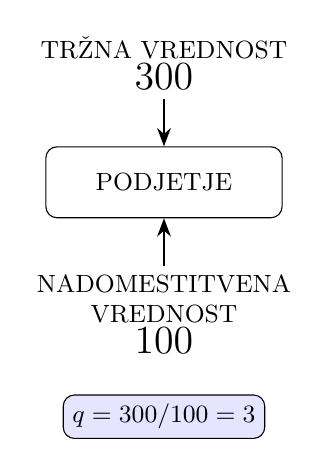
\begin{tikzpicture}[>=Stealth, every node/.style={font=\small}]
\node[align=center] (trg) {TRŽNA VREDNOST\\\Large 300};
\node[draw, rounded corners, minimum width=3cm, minimum height=0.9cm, below=0.6cm of trg] (pod) {PODJETJE};
\node[align=center, below=0.6cm of pod] (nad) {NADOMESTITVENA\\VREDNOST\\\Large 100};
\draw[->, thick] (trg) -- (pod);
\draw[->, thick] (nad) -- (pod);
\node[below=0.4cm of nad, draw, fill=blue!10, rounded corners] {$q = 300 / 100 = 3$};
\end{tikzpicture}
\end{columns}
\end{frame}

% --------------------------------------------------
\begin{frame}{Povezava med q in investicijami}
\note{Čas: ~35--40 s. Amazon (q približno 3,02) in Delta (q približno 0,56). Vprašaj sošolce, katero podjetje ima večjo spodbudo za investiranje. Nato: ali to pomeni, da bo Amazonova investicija bolj donosna? Ne nujno.}
\begin{columns}[T]
\column{0.55\textwidth}
\centering
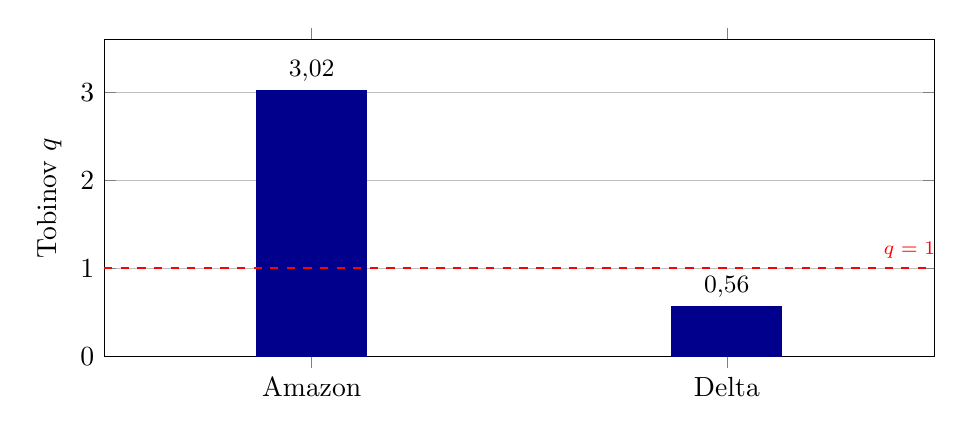
\begin{tikzpicture}
\begin{axis}[
    ybar, bar width=1.4cm,
    width=\textwidth, height=5.6cm,
    ymin=0, ymax=3.6,
    ylabel={Tobinov $q$},
    symbolic x coords={Amazon,Delta},
    xtick=data, enlarge x limits=0.5,
    nodes near coords, nodes near coords align={vertical},
    /pgf/number format/.cd, use comma, fixed, precision=2,
    every node near coord/.append style={font=\small},
    ymajorgrids=true,
]
\addplot[fill=blue!55!black, draw=blue!55!black] coordinates {(Amazon,3.02) (Delta,0.56)};
\draw[dashed, red, thick] (rel axis cs:0,{1/3.6}) -- (rel axis cs:1,{1/3.6}) node[pos=0.97, above, font=\scriptsize, red] {$q=1$};
\end{axis}
\end{tikzpicture}
\column{0.43\textwidth}
\begin{itemize}
\item Amazon: $q = 2.470 / 818 \approx 3{,}02$
\item Delta: $q = 45{,}3 / 81{,}3 \approx 0{,}56$
\item $q>1 \rightarrow$ spodbuda za investicije
\item $q<1 \rightarrow$ manjša spodbuda za investicije
\end{itemize}
\vspace{0.3cm}
\begin{alertblock}{Vprašanje za sošolce}
Katero podjetje bi imelo po tem kazalniku večjo spodbudo za investiranje? Ali to pomeni, da bo tudi bolj donosno?
\end{alertblock}
\end{columns}
\end{frame}

% --------------------------------------------------
\begin{frame}{Tobinov q in investicije v UI}
\note{Čas: ~35--40 s. To je najpomembnejši del: pridemo do dejanske teme. Vprašaj je celotna raziskovalna tema. Tobinov q meri predvsem tržna pričakovanja, ne dejanskega prihodnjega donosa.}
\centering
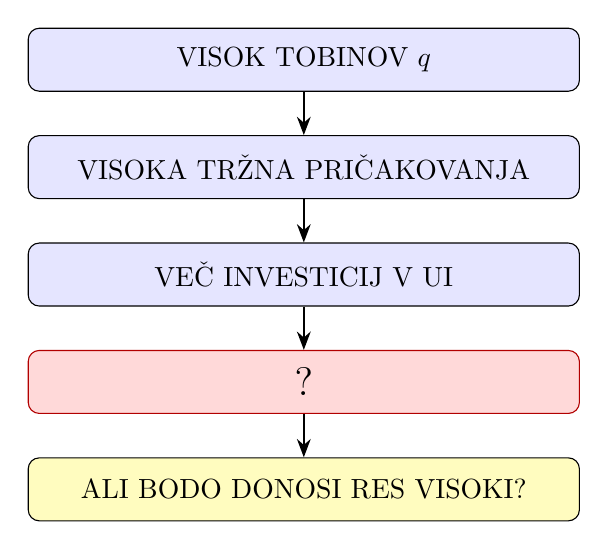
\begin{tikzpicture}[node distance=0.55cm, >=Stealth,
    box/.style={draw, rounded corners, fill=blue!10, minimum width=7cm, minimum height=0.8cm, align=center}]
\node[box] (a) {VISOK TOBINOV $q$};
\node[box, below=of a] (b) {VISOKA TRŽNA PRIČAKOVANJA};
\node[box, below=of b] (c) {VEČ INVESTICIJ V UI};
\node[box, below=of c, fill=red!15, draw=red!70!black] (d) {\Large ?};
\node[box, below=of d, fill=yellow!25] (e) {ALI BODO DONOSI RES VISOKI?};
\draw[->, thick] (a) -- (b);
\draw[->, thick] (b) -- (c);
\draw[->, thick] (c) -- (d);
\draw[->, thick] (d) -- (e);
\end{tikzpicture}
\end{frame}

% --------------------------------------------------
\begin{frame}{Zakaj je q pri UI zanimiv, a omejen}
\note{Čas: ~45--50 s. Izpostavi tri omejitve: (1) visoka tržna vrednost ni visok prihodnji donos, (2) ogromne začetne investicije, (3) neopredmetena sredstva. Zamenjaš lahko ikone s slikami.}
\centering

\begin{tikzpicture}[every node/.style={font=\small}]
% ikona 1: pričakovanja (naraščajoči stolpci)
\begin{scope}[xshift=0cm]
\fill[blue!60!black] (-0.6,0) rectangle (-0.3,0.4);
\fill[blue!60!black] (-0.15,0) rectangle (0.15,0.8);
\fill[blue!60!black] (0.3,0) rectangle (0.6,1.2);
\draw[->, thick, red] (-0.7,0.5) -- (0.7,1.5);
\node[align=center, text width=3.7cm] at (0,-0.8) {\textbf{Pričakovanja}\\Visok $q$ ni dokaz o visokih prihodnjih donosih};
\end{scope}
% ikona 2: podatkovni centri
\begin{scope}[xshift=5cm]
\foreach \y in {0,0.45,0.9}{
  \draw[fill=blue!60!black] (-0.6,\y) rectangle (0.6,\y+0.35);
  \fill[white] (-0.4,\y+0.17) circle (0.05);
  \fill[white] (-0.2,\y+0.17) circle (0.05);
}
\node[align=center, text width=3.7cm] at (0,-0.8) {\textbf{Podatkovni centri}\\Milijarde za čipe in infrastrukturo še ne zagotovijo donosa};
\end{scope}
% ikona 3: neopredmetena sredstva
\begin{scope}[xshift=10cm]
\node[cloud, cloud puffs=9, cloud puff arc=120, aspect=2, draw=blue!60!black, fill=blue!10, thick, minimum width=1.6cm, minimum height=1cm] at (0,0.7) {};
\node at (0,0.7) {\Large ?};
\node[align=center, text width=3.7cm] at (0,-0.8) {\textbf{Neopredmetena sredstva}\\Podatki, algoritmi, znanje: težko merljivi};
\end{scope}
\end{tikzpicture}
\end{frame}

% --------------------------------------------------
\begin{frame}{Kaj nam torej q pove?}
\note{Čas: ~25--30 s. Zaključek: direktno odgovori na naslov teme. Q je dober pokazatelj tržnih pričakovanj, ni pa dovolj za zaključek, da so investicije upravičene.}
\begin{block}{Ali so pričakovanja donosov investicij v UI upravičena?}
Tobinov $q$ je dober pokazatelj \textbf{tržnih pričakovanj}, vendar \textbf{ni dokaz}, da bodo donosi dejansko doseženi.
\end{block}
\begin{itemize}
\item investicije v UI so zelo velike
\item vrednotenje temelji na pričakovanjih
\item pomemben del vrednosti so neopredmetena sredstva
\end{itemize}
\vspace{0.3cm}
\centering
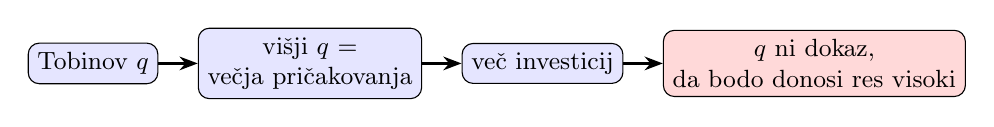
\begin{tikzpicture}[>=Stealth, node distance=0.5cm, every node/.style={font=\small, align=center}]
\node[draw, rounded corners, fill=blue!10] (a) {Tobinov $q$};
\node[draw, rounded corners, fill=blue!10, right=of a] (b) {višji $q$ =\\večja pričakovanja};
\node[draw, rounded corners, fill=blue!10, right=of b] (c) {več investicij};
\node[draw, rounded corners, fill=red!15, right=of c] (d) {$q$ ni dokaz,\\da bodo donosi res visoki};
\draw[->, thick] (a)--(b); \draw[->, thick] (b)--(c); \draw[->, thick] (c)--(d);
\end{tikzpicture}
\end{frame}


% ==================================================
\section{Vedenjski model}
% ==================================================

% --------------------------------------------------
\begin{frame}{Vedenjski model: 1. Postavitev problema}
\begin{itemize}
\item odločanje o obsegu kapitala
\item neoklasična teorija investicij, razširjena s ceno opreme po Jorgensonu
\item gradnja podatkovnih centrov, kupovanje procesorjev GPU in strežnikov ter prodaja storitev UI
\end{itemize}
\begin{block}{Na čem temelji model?}
\begin{enumerate}
\item podjetje je racionalno in maksimizira vrednost premoženja
\item finančni trgi so popolni: podjetje se lahko zadolži po dani obrestni meri $r$
\item proizvodna funkcija $F(K)$ je naraščajoča in konkavna
\item kapital se obrablja po stopnji $\delta$, torej $K_{t+1} = (1-\delta)\cdot K_t + I_t$
\end{enumerate}
\end{block}
\end{frame}

% --------------------------------------------------
\begin{frame}{2. Izpeljava modela}
\begin{itemize}
\item denarni tok $D_t = F(K_t) - I_t - \phi_t$
\item investicije izrazimo iz dinamike kapitala, $I_t = K_{t+1} - (1-\delta)K_t$, odvajamo in dobimo pogoj prvega reda:
\end{itemize}
\[
\boxed{F'(K_{t+1}) = r + \delta}
\]
\begin{itemize}
\item najemni strošek $R = r + \delta$, maksimiziranje dobička $\pi = F(K) - R\cdot K$
\item dokler dodatna enota kapitala prinese več (mejni produkt kapitala, MPK), kot stane ($R$), se podjetju splača dodajati kapital
\item če MPK $> R$: premalo kapitala; če MPK $< R$: preveč kapitala
\end{itemize}
\end{frame}

% --------------------------------------------------
\begin{frame}{Razširitev: cena opreme}
\begin{itemize}
\item cene računalniške opreme se spreminjajo! Zato najemni strošek razširimo in izrazimo v enotah izdelka:
\end{itemize}
\[
\boxed{R = \frac{P_K}{P}\,(r + \delta - \pi_K)}
\]
\begin{itemize}
\item $r$: oportunitetni strošek vloženih sredstev (vključno s premijo za tveganje)
\item $\delta$: del kapitala, ki se v enem letu izrabi ali zastara in ga je treba nadomestiti
\item $\pi_K$: pričakovana sprememba cene kapitala
\item amortizacija, cenovna gibanja
\end{itemize}
\end{frame}

% --------------------------------------------------
\begin{frame}{Želena zaloga kapitala in investicije}
\begin{itemize}
\item $F(K) = A\cdot K^{\gamma}$, MPK $= \gamma\cdot A\cdot K^{\gamma-1}$, kjer je $A$ produktivnost podjetja
\item če to izenačimo z $R$, dobimo želeno (optimalno) zalogo kapitala:
\end{itemize}
\[
\boxed{K^{*} = \left(\frac{\gamma\cdot A}{R}\right)^{\frac{1}{1-\gamma}}}
\]
\begin{itemize}
\item bruto investicije so razlika med želeno zalogo v naslednjem obdobju in kapitalom, ki ostane po amortizaciji:
\end{itemize}
\[
\boxed{I_t = K^{*}_{t+1} - (1-\delta)\cdot K_t}
\]
\begin{itemize}
\item investicije: (1) nadomestitev obrabljenega kapitala ($\delta\cdot K$), (2) neto povečanje zaloge proti želeni ravni
\end{itemize}
\end{frame}

% --------------------------------------------------
\begin{frame}{3. Numerični primer: Microsoftove naložbe v UI}
\begin{itemize}
\item nabave osnovnih sredstev v drugi polovici leta 2025
\item Microsoftov podatkovni center Fairwater v Wisconsinu (prva faza 3,3 mrd \$, druga še 4 mrd \$)
\end{itemize}
\begin{table}
\centering
\scriptsize
\setlength{\tabcolsep}{3pt}
\renewcommand{\arraystretch}{1.15}
\begin{tabular}{L{3.9cm}R{1.2cm}R{1.5cm}R{0.9cm}R{1.2cm}R{1.2cm}R{1.3cm}R{2.4cm}}
\toprule
\textbf{Vrsta kapitala} & \textbf{Delež nabav} & \textbf{Vrednost (mrd \$)} & $r$ & $\delta$ & $\pi_K$ & $R$ & \textbf{Zahtevani donos (mrd \$/leto)} \\
\midrule
Računalniška oprema (strežniki, GPU) & 57~\% & 38,8 & 8~\% & 16,7~\% & $-5$~\% & 29,7~\% & 11,5 \\
Zgradbe in izboljšave & 39~\% & 26,5 & 8~\% & 6,7~\% & $+2$~\% & 12,7~\% & 3,4 \\
\midrule
Skupaj (brez 4~\% drugo) & 96~\% & 65,3 & & & & 22,8~\% & 14,9 \\
\bottomrule
\end{tabular}
\caption{Nabave osnovnih sredstev Microsofta, julij--december 2025 (skupaj 68 mrd \$), in zahtevani donos. Viri: nabave in delitev: Epoch AI (2026) po Microsoftovem 10-K/10-Q (Opomba 6); $r$: FRED, DFII10 (okoli 2~\%) plus predpostavljena premija za tveganje 6 o.\,t.; $\delta$: Microsoft 10-K (strežniki 2--6 let, zgradbe 5--15 let; $\delta = 1/6$ oziroma $1/15$); $\pi_K$ opreme: BLS, PPI PCU33413341 (dolgoročni povprečni padec okoli 5~\% na leto); $\pi_K$ zgradb: predpostavka. Lastni izračun.}
\end{table}
\end{frame}

% --------------------------------------------------
\begin{frame}{Zahtevani donos in prihodki iz UI}
\begin{columns}[T]
\column{0.52\textwidth}
\begin{figure}
\centering
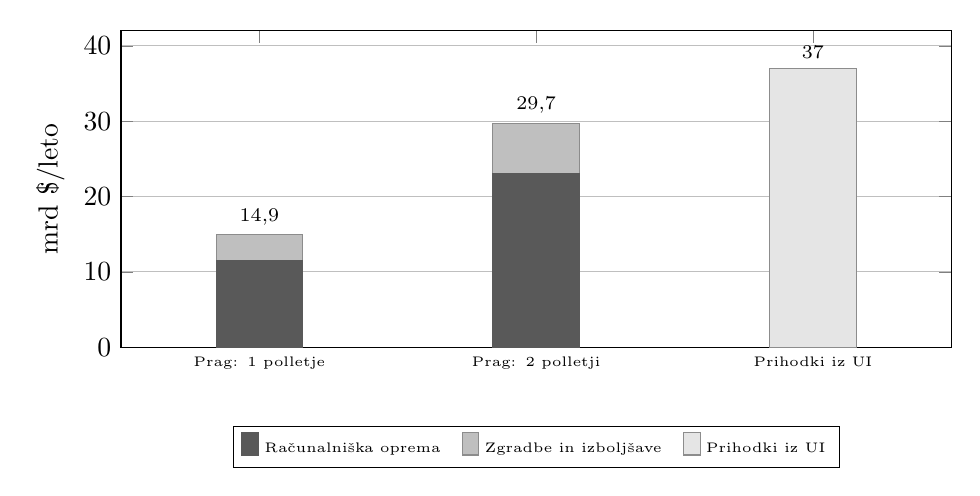
\begin{tikzpicture}
\begin{axis}[
    ybar stacked, bar width=1.1cm,
    width=\textwidth, height=5.6cm,
    ymin=0, ymax=42,
    ylabel={mrd \$/leto},
    symbolic x coords={enega,dveh,prihodki},
    xtick=data,
    xticklabels={Prag: 1 polletje, Prag: 2 polletji, Prihodki iz UI},
    xticklabel style={align=center, text width=1.8cm, font=\tiny},
    enlarge x limits=0.25,
    ymajorgrids=true,
    legend style={at={(0.5,-0.25)}, anchor=north, legend columns=-1, font=\tiny, /tikz/every even column/.append style={column sep=0.2cm}},
]
\addplot+[fill=black!65, draw=black!65] coordinates {(enega,11.5) (dveh,23.0) (prihodki,0)};
\addplot+[fill=black!25, draw=black!45] coordinates {(enega,3.4) (dveh,6.7) (prihodki,0)};
\addplot+[fill=black!10, draw=black!45] coordinates {(enega,0) (dveh,0) (prihodki,37)};
\legend{Računalniška oprema, Zgradbe in izboljšave, Prihodki iz UI}
\node[above] at (axis cs:enega,14.9) {\scriptsize 14,9};
\node[above] at (axis cs:dveh,29.7) {\scriptsize 29,7};
\node[above] at (axis cs:prihodki,37) {\scriptsize 37};
\end{axis}
\end{tikzpicture}
\caption{Zahtevani donos na nabave in prihodki Microsofta iz UI. Viri: Tabela 1, lastni izračun; prihodki iz UI: Microsoft, rezultati za FY2026 Q3 (29. 4. 2026), letna stopnja prihodkov 37 mrd \$.}
\end{figure}
\column{0.46\textwidth}
\scriptsize
\begin{itemize}
\item oprema: 57~\% nabav, 77~\% donosa (visok $R$ v primerjavi z zgradbami)
\item nabave iz polletja morajo vsako leto ustvariti 14,9 mrd \$ donosa; v naslednjem polletju bi prag znašal okoli 30 mrd \$ na leto
\item prihodki iz UI (marec 2026) so dosegli letno stopnjo 37 mrd \$ (123~\% več kot leto prej); prag za nabave iz dveh polletij (30 mrd \$) je okoli 80~\% teh prihodkov
\item prag je neto donos kapitala, prihodki iz UI pa so bruto; poleg tega nabave niso v celoti namenjene UI
\item prihodki iz UI morajo hitro rasti, da bi pokrili prag, ki ga ustvarjajo nabave opreme
\end{itemize}
\end{columns}
\end{frame}

% --------------------------------------------------
\begin{frame}{Občutljivost}
\begin{table}
\centering
\scriptsize
\renewcommand{\arraystretch}{1.15}
\setlength{\tabcolsep}{4pt}
\begin{tabular}{L{6.2cm}R{1.7cm}R{3.0cm}R{1.8cm}}
\toprule
\textbf{Scenarij (ostali parametri kot v izhodišču)} & \textbf{$R$ opreme} & \textbf{Zahtevani donos (mrd \$/leto)} & \textbf{Sprememba} \\
\midrule
Izhodišče ($r = 8$~\%, $\delta = 16{,}7$~\%, $\pi_K = -5$~\%) & 29,7~\% & 14,9 & -- \\
$r = 2$~\% (brez premije za tveganje) & 23,7~\% & 10,9 & $-26$~\% \\
$\pi_K = +4{,}2$~\% (cene opreme v 2025) & 20,5~\% & 11,3 & $-24$~\% \\
Življenjska doba 3 leta ($\delta = 33{,}3$~\%) & 46,3~\% & 21,3 & $+44$~\% \\
\bottomrule
\end{tabular}
\caption{Občutljivost zahtevanega donosa na parametre (lastni izračun po modelu, osnova: Tabela 1).}
\end{table}
\begin{itemize}
\item prag je najbolj občutljiv na življenjsko dobo opreme: 3 leta namesto 6 $\rightarrow$ $+44$~\%
\item odprava premije za tveganje $\rightarrow$ $-26$~\%, rast cen opreme $\rightarrow$ $-24$~\%
\item prag se giblje med 10,9 in 21,3 mrd \$, torej se razlikuje za skoraj dvakrat
\end{itemize}
\end{frame}

% --------------------------------------------------
\begin{frame}{Primeri iz prakse: koliko časa služi oprema za UI?}
\begin{itemize}
\item vrednost $\delta$ za opremo podjetja ocenjujejo z računovodsko življenjsko dobo
\end{itemize}
\begin{table}
\centering
\scriptsize
\renewcommand{\arraystretch}{1.15}
\setlength{\tabcolsep}{4pt}
\begin{tabular}{L{4.2cm}R{1.2cm}R{1.5cm}R{2.8cm}R{3.0cm}}
\toprule
\textbf{Življenjska doba opreme} & $\delta$ & \textbf{$R$ opreme} & \textbf{Zahtevani donos (mrd \$/leto)} & \textbf{Sprememba glede na 6 let} \\
\midrule
6 let (Microsoft, Alphabet, Oracle) & 16,7~\% & 29,7~\% & 14,9 & -- \\
5,5 leta (Meta) & 18,2~\% & 31,2~\% & 15,5 & $+0{,}6$ mrd \$ ($+4$~\%) \\
5 let (Amazon, del opreme) & 20,0~\% & 33,0~\% & 16,1 & $+1{,}3$ mrd \$ ($+9$~\%) \\
4 leta & 25,0~\% & 38,0~\% & 18,1 & $+3{,}2$ mrd \$ ($+22$~\%) \\
3 leta (Burry) & 33,3~\% & 46,3~\% & 21,3 & $+6{,}5$ mrd \$ ($+44$~\%) \\
\bottomrule
\end{tabular}
\caption{Zahtevani donos na nabave iz Tabele 1 glede na življenjsko dobo opreme (lastni izračun po modelu; življenjske dobe iz 10-K poročil podjetij in javnih izjav).}
\end{table}
\end{frame}

\begin{frame}{Primeri iz prakse: kaj pomenijo ocene življenjske dobe?}
\begin{itemize}
\item prag donosa se z vsakim letom krajše življenjske dobe zviša (vse hitreje)
\item razlika med ocenami podjetij (5 do 6 let): eno leto krajša doba zviša prag za 1,3 mrd \$, kar je enako učinku dveh odstotnih točk višje obrestne mere
\item razlika med uradnimi ocenami in Burryjevo: prag za 44~\% višji
\item prag donosa je torej močno odvisen od ocene življenjske dobe, ki jo podjetja same določajo
\end{itemize}
\end{frame}

% --------------------------------------------------
\begin{frame}{4. Ali so pričakovanja donosov upravičena? Prag rentabilnosti}
\begin{itemize}
\item naložba je upravičena, če je donos kapitala vsaj enak najemnemu strošku
\end{itemize}
\begin{table}
\centering
\scriptsize
\renewcommand{\arraystretch}{1.15}
\setlength{\tabcolsep}{4pt}
\begin{tabular}{L{5.2cm}R{2.7cm}R{2.7cm}R{3.0cm}}
\toprule
\textbf{Scenarij} & \textbf{Prag za nabave enega polletja (mrd \$)} & \textbf{Prag ob dveh polletjih (mrd \$)} & \textbf{Prag kot delež prihodkov iz UI (37 mrd \$)} \\
\midrule
Optimistični ($r = 2$~\%, $\pi_K = +4{,}2$~\%) & 7,4 & 14,8 & 40~\% \\
Osnovni ($r = 8$~\%, $\delta = 16{,}7$~\%, $\pi_K = -5$~\%) & 14,9 & 29,7 & 80~\% \\
Pesimistični ($r = 10$~\%, $\delta = 33{,}3$~\%) & 22,6 & 45,2 & 122~\% \\
\bottomrule
\end{tabular}
\caption{Test upravičenosti naložb Microsofta v UI (lastni izračun; prihodki iz UI: Microsoft, rezultati za FY2026 Q3, letna stopnja 37 mrd \$).}
\end{table}
\footnotesize
\begin{itemize}
\item v optimističnem scenariju kapital ustvari 40~\% prihodkov iz UI, v osnovnem 80~\%, v pesimističnem 122~\%
\item pričakovanja donosov so torej upravičena le, če prihodki iz UI še naprej hitro rastejo (v zadnjem letu so se več kot podvojili; 123~\%); če se podvojijo še enkrat, bi osnovni prag znašal okoli 40~\% prihodkov
\item pri slabših predpostavkah o življenjski dobi in premiji za tveganje pa že današnja raven prihodkov ne bi zadoščala
\end{itemize}
\end{frame}

% --------------------------------------------------
\begin{frame}{5. Ireverzibilnost investicij}
\begin{itemize}
\item predpostavka osnovnega modela: podjetje lahko kapital kadar koli proda
\item tu je drugače: del investicije je pogosto izgubljen (angl. \textit{sunk cost}): $F'(K) < r + \delta$ (kapitala je preveč, a ga podjetje ne more prodati)
\item specializirani procesorji se težko preprodajo po prvotni vrednosti
\item optična vlakna: tudi tam je bilo naložb preveč, a je kapital z nizko amortizacijo obstal in so ga izkoristili drugi
\end{itemize}
\begin{alertblock}{Sklep}
Pri GPU z visokim $\delta$ napačna ocena povpraševanja pomeni hitro izgubo vrednosti, zato je tveganje preinvestiranja večje.
\end{alertblock}
\end{frame}


% ==================================================
% ZAKLJUČEK  (prosojnice za zaključek pridejo sem)
% ==================================================

\end{document}